\chapter{Конструкторская часть}

В данном разделе будут представлены схемы алгоритмов поиска в словаре: полного перебора, бинарного поиска и поиска сегментами. Будут описаны типы и структуры данных, используемые для реализации, а также структура разрабатываемого программного обеспечения. Кроме того, будут выделены классы эквивалентности для тестирования.

\section{Разработка алгоритмов}

На рисунке \ref{img:brute} приведена схема алгоритма поиска в словаре полным перебором. Схема бинарного поиска приведена на рисунке \ref{img:binary}. Схема сегментного поиска показана на рисунке \ref{img:segment}.

\begin{figure}[H]
	\begin{center}
		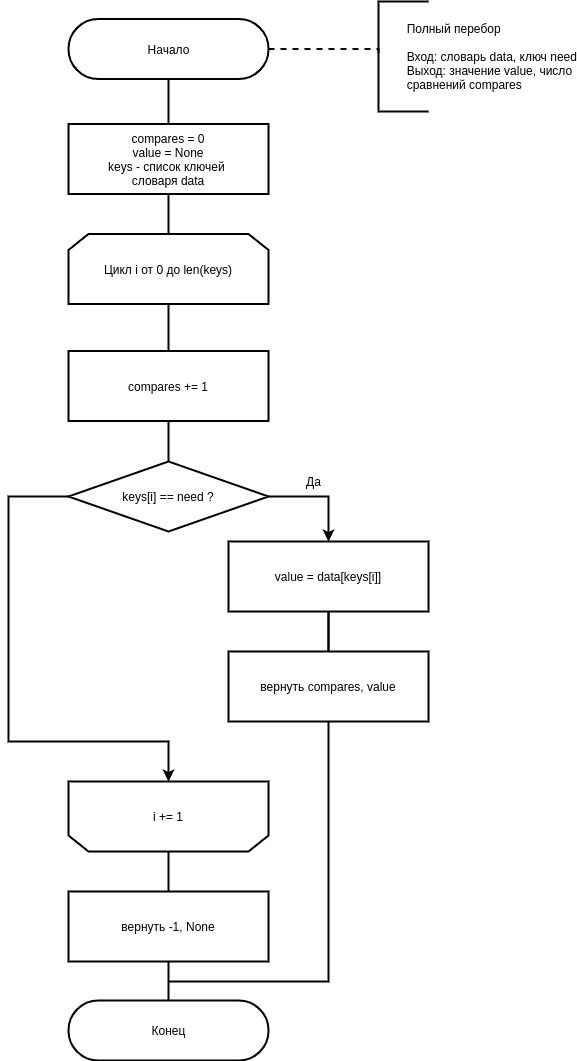
\includegraphics[scale=0.6]{img/brute_force.png}
	\end{center}
	\captionsetup{justification=centering}
	\caption{Полный перебор}
	\label{img:brute}
\end{figure}

\begin{figure}[H]
	\begin{center}
		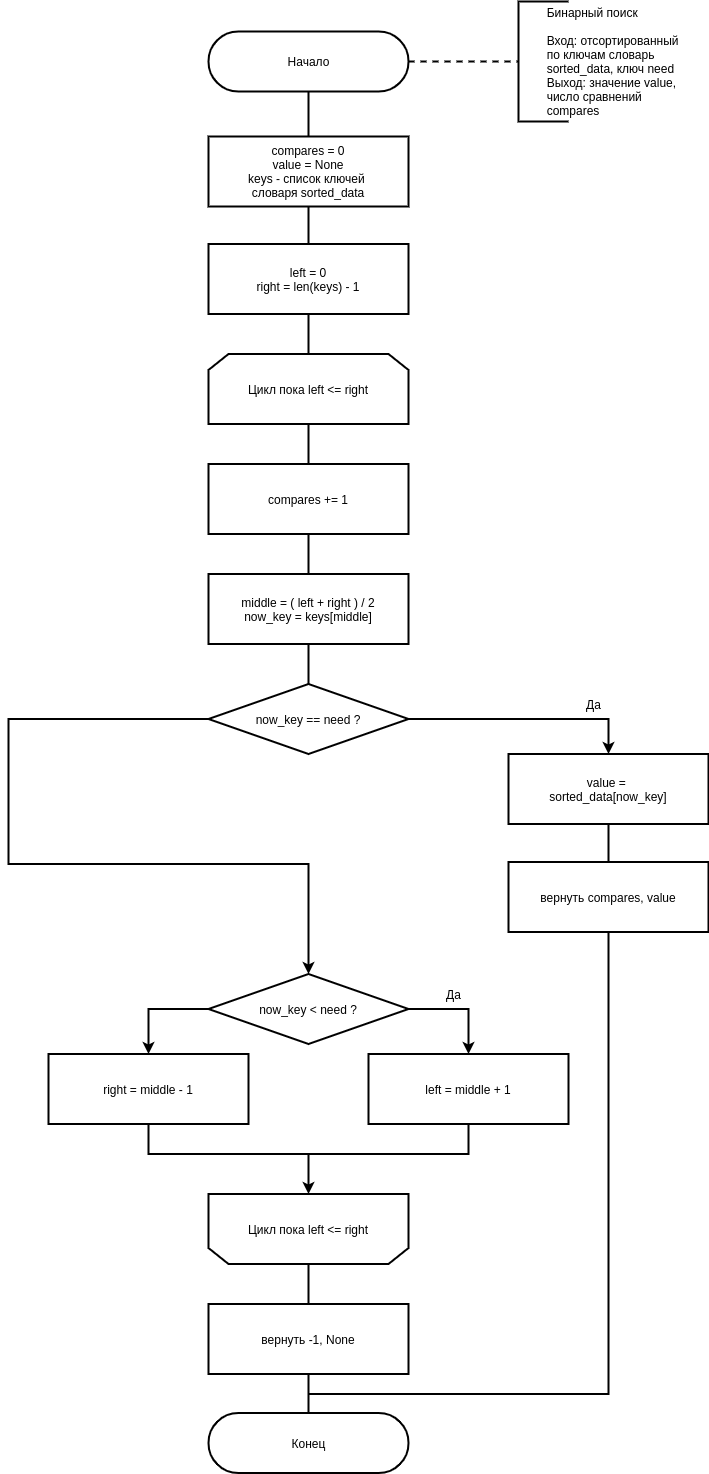
\includegraphics[scale=0.4]{img/binary.png}
	\end{center}
	\captionsetup{justification=centering}
	\caption{Бинарный поиск}
	\label{img:binary}
\end{figure}

\begin{figure}[H]
	\begin{center}
		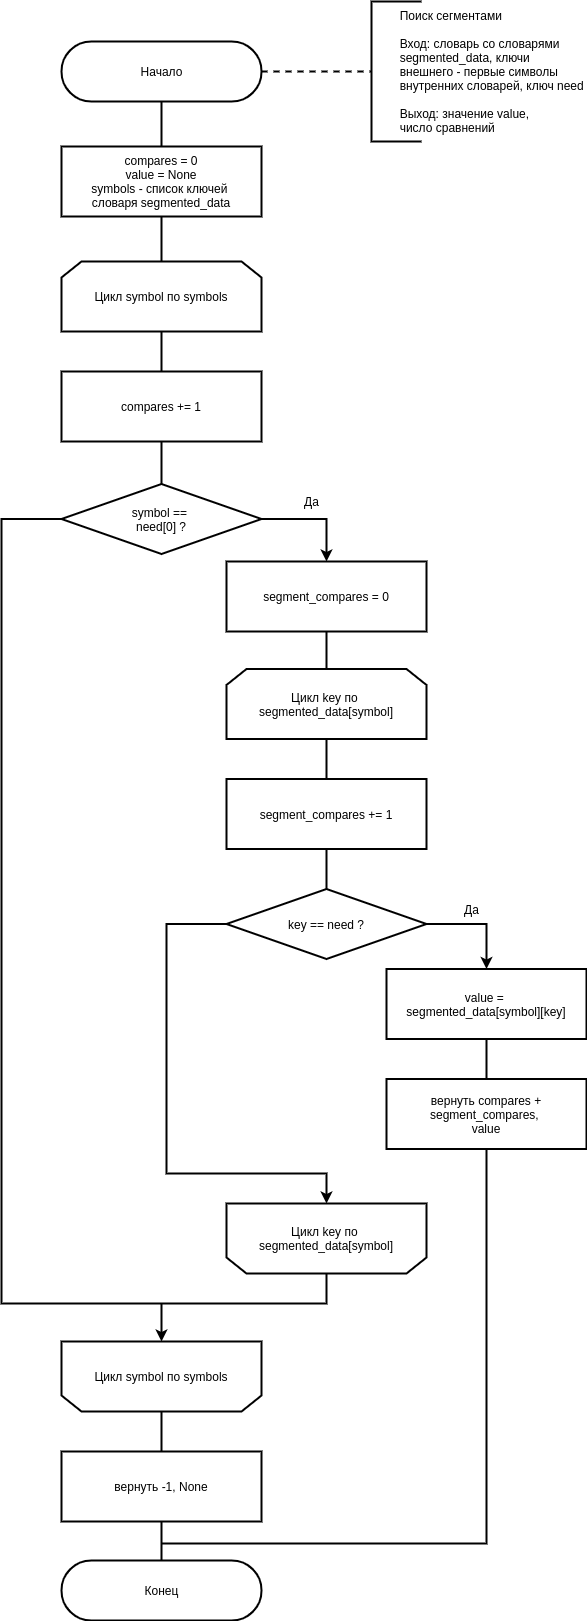
\includegraphics[scale=0.4]{img/segment.png}
	\end{center}
	\captionsetup{justification=centering}
	\caption{Поиск сегментами}
	\label{img:segment}
\end{figure}

\section{Описание используемых типов и структур данных}

Для реализации словаря будет использован встроенный тип данных $dict$ в $Python$, при этом для задания ключа и значения будет использован тип данных $str$.

Для числа сравнений будет использован тип данных $int$.

\section{Структура разрабатываемого ПО}

При реализации разрабатываемого программного обеспечения будет использоваться метод структурного программирования. Для взаимодействия с пользователем будет выделена функция $process()$, из которой будут вызываться методы поиска в словаре и функции сравнительного анализа. Методы поиска в словаре будут реализованы в следующих функциях, входные параметры которых - ключ, по которому происходит поиск, и словарь значений, а выходные параметры - число сравнений и найденное по ключу значение:
\begin{itemize}
	\item функция полного перебора;
	\item функция бинарного поиска;
	\item функция поиска сегментами.
\end{itemize}

Для работы со словарем будут разработаны следующие функции:

\begin{itemize}
	\item загрузка данных в словарь из файла, входной параметр - имя файла, выходный - заполненный словарь значений;
	\item сортировка словаря по ключам, входной параметр - словарь значений, выходной - отсортированный по ключам словарь;
	\item сортировка словаря по значениям, входной параметр - словарь значений, выходной - отсортированный по значениям словарь;
	\item вывод словаря, входной параметр - словарь значений, выходной - вывод пар ключ-значение на экран. 
\end{itemize}

Для сравнительного анализа будут реализованы:

\begin{itemize}
	\item функция замеров времени, выходным параметром которой является массив временных значений;
	\item функция замеров числа сравнений, выходным параметром которой является массив числа сравнений;
	\item функция графического представления замеров времени, у которой на входе - массив временных значений или массив числа сравнений, на выходе - графическое представление.
\end{itemize}

\section{Классы эквивалентности при тестировании}

Для тестирования разрабатываемой программы будут выделены следующие классы эквивалентности:

\begin{itemize}
	\item неверный ввод ключа - пустое значение;
	\item введенного ключа нет в словаре;
	\item введенный ключ есть в словаре.
\end{itemize}

\section{Вывод}

Были представлены схемы поиска в словаре. Были указаны типы и структуры данных, используемые для реализации, и описана структура разрабатываемого программного обеспечения. Также были выделены классы эквивалентности для тестирования ПО.
